\documentclass{standalone}
\usepackage{tikz}
\usetikzlibrary{patterns, positioning}

\begin{document}
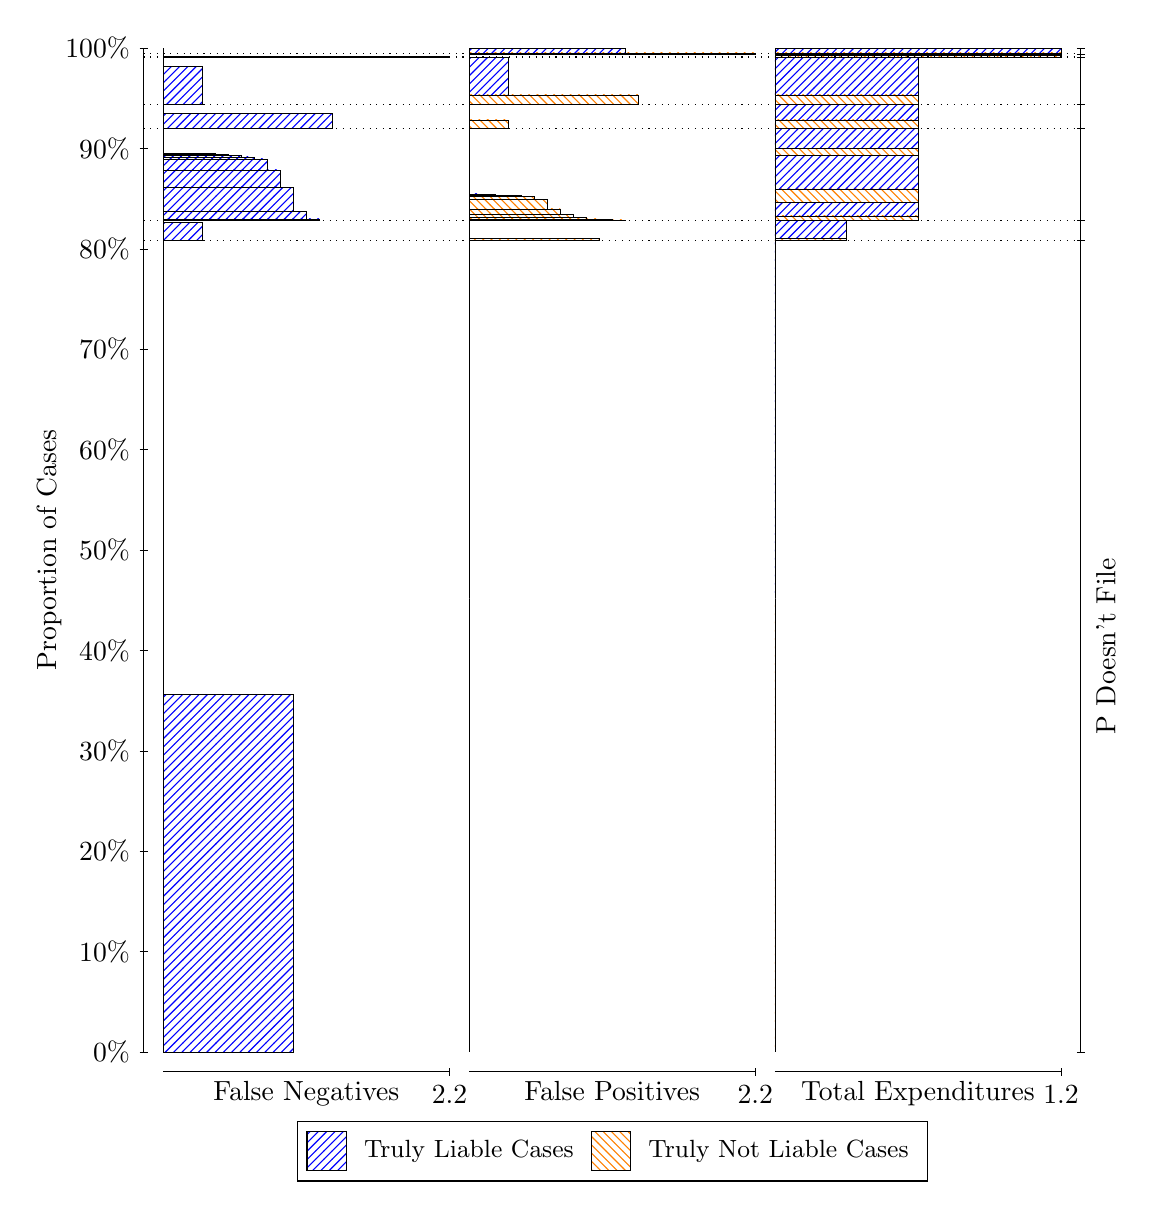
\begin{tikzpicture}
\draw[black, very thin] (1.5,1.75) -- (1.5,14.5);
\node[rotate=90, anchor=center] at (0.3, 8.125) {Proportion of Cases};
\draw[black, very thin] (1.45,1.75) -- (1.55,1.75);
\node[anchor=east] at (1.45, 1.75) {0\%};
\draw[black, very thin] (1.45,3.025) -- (1.55,3.025);
\node[anchor=east] at (1.45, 3.025) {10\%};
\draw[black, very thin] (1.45,4.3) -- (1.55,4.3);
\node[anchor=east] at (1.45, 4.3) {20\%};
\draw[black, very thin] (1.45,5.575) -- (1.55,5.575);
\node[anchor=east] at (1.45, 5.575) {30\%};
\draw[black, very thin] (1.45,6.85) -- (1.55,6.85);
\node[anchor=east] at (1.45, 6.85) {40\%};
\draw[black, very thin] (1.45,8.125) -- (1.55,8.125);
\node[anchor=east] at (1.45, 8.125) {50\%};
\draw[black, very thin] (1.45,9.4) -- (1.55,9.4);
\node[anchor=east] at (1.45, 9.4) {60\%};
\draw[black, very thin] (1.45,10.675) -- (1.55,10.675);
\node[anchor=east] at (1.45, 10.675) {70\%};
\draw[black, very thin] (1.45,11.95) -- (1.55,11.95);
\node[anchor=east] at (1.45, 11.95) {80\%};
\draw[black, very thin] (1.45,13.225) -- (1.55,13.225);
\node[anchor=east] at (1.45, 13.225) {90\%};
\draw[black, very thin] (1.45,14.5) -- (1.55,14.5);
\node[anchor=east] at (1.45, 14.5) {100\%};

\draw[black, very thin] (13.4,1.75) -- (13.4,14.5);
\draw[black, very thin] (13.35,1.75) -- (13.45,1.75);
\node[anchor=west] at (13.35, 1.75) {};
\draw[black, very thin] (13.35,12.058) -- (13.45,12.058);
\node[anchor=west] at (13.35, 12.058) {};
\draw[black, very thin] (13.35,12.312) -- (13.45,12.312);
\node[anchor=west] at (13.35, 12.312) {};
\draw[black, very thin] (13.35,13.475) -- (13.45,13.475);
\node[anchor=west] at (13.35, 13.475) {};
\draw[black, very thin] (13.35,13.784) -- (13.45,13.784);
\node[anchor=west] at (13.35, 13.784) {};
\draw[black, very thin] (13.35,14.386) -- (13.45,14.386);
\node[anchor=west] at (13.35, 14.386) {};
\draw[black, very thin] (13.35,14.426) -- (13.45,14.426);
\node[anchor=west] at (13.35, 14.426) {};
\draw[black, very thin] (13.35,14.5) -- (13.45,14.5);
\node[anchor=west] at (13.35, 14.5) {};

\draw[black, very thin, pattern color=blue, pattern=north east lines] (1.75,1.75) rectangle (3.4015,6.2956);
\draw[black, very thin, pattern color=orange, pattern=north west lines] (1.75,6.2956) rectangle (1.75,12.058);
\draw[black, very thin, pattern color=blue, pattern=north east lines] (1.75,12.058) rectangle (2.2455,12.289);
\draw[black, very thin, pattern color=orange, pattern=north west lines] (1.75,12.289) rectangle (1.75,12.312);
\draw[black, very thin, pattern color=blue, pattern=north east lines] (1.75,12.312) rectangle (3.7318,12.329);
\draw[black, very thin, pattern color=blue, pattern=north east lines] (1.75,12.329) rectangle (3.5667,12.426);
\draw[black, very thin, pattern color=blue, pattern=north east lines] (1.75,12.426) rectangle (3.4015,12.727);
\draw[black, very thin, pattern color=blue, pattern=north east lines] (1.75,12.727) rectangle (3.2364,12.737);
\draw[black, very thin, pattern color=blue, pattern=north east lines] (1.75,12.737) rectangle (3.2364,12.951);
\draw[black, very thin, pattern color=blue, pattern=north east lines] (1.75,12.951) rectangle (3.0712,13.092);
\draw[black, very thin, pattern color=blue, pattern=north east lines] (1.75,13.092) rectangle (2.9061,13.118);
\draw[black, very thin, pattern color=blue, pattern=north east lines] (1.75,13.118) rectangle (2.7409,13.138);
\draw[black, very thin, pattern color=blue, pattern=north east lines] (1.75,13.138) rectangle (2.5758,13.147);
\draw[black, very thin, pattern color=blue, pattern=north east lines] (1.75,13.147) rectangle (2.4106,13.158);
\draw[black, very thin, pattern color=orange, pattern=north west lines] (1.75,13.158) rectangle (1.75,13.475);
\draw[black, very thin, pattern color=blue, pattern=north east lines] (1.75,13.475) rectangle (3.897,13.673);
\draw[black, very thin, pattern color=orange, pattern=north west lines] (1.75,13.673) rectangle (1.75,13.784);
\draw[black, very thin, pattern color=blue, pattern=north east lines] (1.75,13.784) rectangle (2.2455,14.264);
\draw[black, very thin, pattern color=orange, pattern=north west lines] (1.75,14.264) rectangle (1.75,14.386);
\draw[black, very thin, pattern color=blue, pattern=north east lines] (1.75,14.386) rectangle (5.3833,14.398);
\draw[black, very thin, pattern color=orange, pattern=north west lines] (1.75,14.398) rectangle (1.75,14.426);
\draw[black, very thin, pattern color=orange, pattern=north west lines] (1.75,14.426) rectangle (1.75,14.439);
\draw[black, very thin, pattern color=blue, pattern=north east lines] (1.75,14.439) rectangle (1.75,14.5);
\draw[black, very thin, pattern color=orange, pattern=north west lines] (5.6333,1.75) rectangle (5.6333,7.512);
\draw[black, very thin, pattern color=blue, pattern=north east lines] (5.6333,7.512) rectangle (5.6333,12.058);
\draw[black, very thin, pattern color=orange, pattern=north west lines] (5.6333,12.058) rectangle (7.2848,12.08);
\draw[black, very thin, pattern color=blue, pattern=north east lines] (5.6333,12.08) rectangle (5.6333,12.312);
\draw[black, very thin, pattern color=orange, pattern=north west lines] (5.6333,12.312) rectangle (7.6152,12.317);
\draw[black, very thin, pattern color=orange, pattern=north west lines] (5.6333,12.317) rectangle (7.45,12.322);
\draw[black, very thin, pattern color=orange, pattern=north west lines] (5.6333,12.322) rectangle (7.2848,12.33);
\draw[black, very thin, pattern color=orange, pattern=north west lines] (5.6333,12.33) rectangle (7.1197,12.345);
\draw[black, very thin, pattern color=orange, pattern=north west lines] (5.6333,12.345) rectangle (6.9545,12.387);
\draw[black, very thin, pattern color=orange, pattern=north west lines] (5.6333,12.387) rectangle (6.7894,12.458);
\draw[black, very thin, pattern color=orange, pattern=north west lines] (5.6333,12.458) rectangle (6.6242,12.575);
\draw[black, very thin, pattern color=orange, pattern=north west lines] (5.6333,12.575) rectangle (6.4591,12.613);
\draw[black, very thin, pattern color=orange, pattern=north west lines] (5.6333,12.613) rectangle (6.2939,12.628);
\draw[black, very thin, pattern color=blue, pattern=north east lines] (5.6333,12.628) rectangle (5.9636,12.639);
\draw[black, very thin, pattern color=blue, pattern=north east lines] (5.6333,12.639) rectangle (5.7985,12.648);
\draw[black, very thin, pattern color=blue, pattern=north east lines] (5.6333,12.648) rectangle (5.6333,13.475);
\draw[black, very thin, pattern color=orange, pattern=north west lines] (5.6333,13.475) rectangle (6.1288,13.586);
\draw[black, very thin, pattern color=blue, pattern=north east lines] (5.6333,13.586) rectangle (5.6333,13.784);
\draw[black, very thin, pattern color=orange, pattern=north west lines] (5.6333,13.784) rectangle (7.7803,13.906);
\draw[black, very thin, pattern color=blue, pattern=north east lines] (5.6333,13.906) rectangle (6.1288,14.386);
\draw[black, very thin, pattern color=orange, pattern=north west lines] (5.6333,14.386) rectangle (5.6333,14.414);
\draw[black, very thin, pattern color=blue, pattern=north east lines] (5.6333,14.414) rectangle (5.6333,14.426);
\draw[black, very thin, pattern color=orange, pattern=north west lines] (5.6333,14.426) rectangle (9.2667,14.439);
\draw[black, very thin, pattern color=blue, pattern=north east lines] (5.6333,14.439) rectangle (7.6152,14.5);
\draw[black, very thin, pattern color=orange, pattern=north west lines] (9.5167,1.75) rectangle (9.5167,7.512);
\draw[black, very thin, pattern color=blue, pattern=north east lines] (9.5167,7.512) rectangle (9.5167,12.058);
\draw[black, very thin, pattern color=orange, pattern=north west lines] (9.5167,12.058) rectangle (10.425,12.08);
\draw[black, very thin, pattern color=blue, pattern=north east lines] (9.5167,12.08) rectangle (10.425,12.312);
\draw[black, very thin, pattern color=orange, pattern=north west lines] (9.5167,12.312) rectangle (11.333,12.367);
\draw[black, very thin, pattern color=blue, pattern=north east lines] (9.5167,12.367) rectangle (11.333,12.537);
\draw[black, very thin, pattern color=orange, pattern=north west lines] (9.5167,12.537) rectangle (11.333,12.71);
\draw[black, very thin, pattern color=blue, pattern=north east lines] (9.5167,12.71) rectangle (11.333,13.136);
\draw[black, very thin, pattern color=orange, pattern=north west lines] (9.5167,13.136) rectangle (11.333,13.224);
\draw[black, very thin, pattern color=blue, pattern=north east lines] (9.5167,13.224) rectangle (11.333,13.475);
\draw[black, very thin, pattern color=orange, pattern=north west lines] (9.5167,13.475) rectangle (11.333,13.586);
\draw[black, very thin, pattern color=blue, pattern=north east lines] (9.5167,13.586) rectangle (11.333,13.784);
\draw[black, very thin, pattern color=orange, pattern=north west lines] (9.5167,13.784) rectangle (11.333,13.906);
\draw[black, very thin, pattern color=blue, pattern=north east lines] (9.5167,13.906) rectangle (11.333,14.386);
\draw[black, very thin, pattern color=orange, pattern=north west lines] (9.5167,14.386) rectangle (13.15,14.414);
\draw[black, very thin, pattern color=blue, pattern=north east lines] (9.5167,14.414) rectangle (13.15,14.426);
\draw[black, very thin, pattern color=orange, pattern=north west lines] (9.5167,14.426) rectangle (13.15,14.439);
\draw[black, very thin, pattern color=blue, pattern=north east lines] (9.5167,14.439) rectangle (13.15,14.5);
\draw[black, dotted] (1.5,12.058) -- (13.4,12.058);
\draw[black, dotted] (1.5,12.312) -- (13.4,12.312);
\draw[black, dotted] (1.5,13.475) -- (13.4,13.475);
\draw[black, dotted] (1.5,13.784) -- (13.4,13.784);
\draw[black, dotted] (1.5,14.386) -- (13.4,14.386);
\draw[black, dotted] (1.5,14.426) -- (13.4,14.426);
\draw[black, very thin] (1.75,1.5) -- (5.3833,1.5);
\node[anchor=north] at (3.5667, 1.5) {False Negatives};
\draw[black, very thin] (5.3833,1.45) -- (5.3833,1.55);
\node[anchor=north] at (5.3833, 1.45) {2.2};

\draw[black, very thin] (5.6333,1.5) -- (9.2667,1.5);
\node[anchor=north] at (7.45, 1.5) {False Positives};
\draw[black, very thin] (9.2667,1.45) -- (9.2667,1.55);
\node[anchor=north] at (9.2667, 1.45) {2.2};

\draw[black, very thin] (9.5167,1.5) -- (13.15,1.5);
\node[anchor=north] at (11.333, 1.5) {Total Expenditures};
\draw[black, very thin] (13.15,1.45) -- (13.15,1.55);
\node[anchor=north] at (13.15, 1.45) {1.2};

\node[black, centered, rotate=90] at (13.72, 6.9038) {P Doesn't File};







\draw (7.449999999999999,1.5) node[draw=none] (baseCoordinate) {};
\begin{scope}[align=center]
        \matrix[scale=0.5, draw=black, below=0.5cm of baseCoordinate, nodes={draw}, column sep=0.1cm]{
            \node[rectangle, draw, minimum width=0.5cm, minimum height=0.5cm, pattern=north east lines, pattern color=blue] {}; &
            \node[draw=none, font=\small] (B) {Truly Liable Cases}; &
            \node[rectangle, draw, minimum width=0.5cm, minimum height=0.5cm, pattern=north west lines, pattern color=orange] {}; &
            \node[draw=none, font=\small] (B) {Truly Not Liable Cases}; \\
            };
\end{scope}

\end{tikzpicture}
\end{document}